\documentclass[aspectratio=169]{beamer}

% For presentation mode with notes on second screen:
\setbeameroption{show notes on second screen=right}
% For final PDF without notes, comment above line and uncomment below:
% \setbeameroption{hide notes}

\usepackage[utf8]{inputenc}
\usepackage{amsmath}
\usepackage{amsfonts}
\usepackage{amssymb}
\usepackage{graphicx}
\usepackage{ragged2e}  % `\justifying` text
\usepackage{booktabs}  % Tables
\usepackage{tabularx}
\usepackage{tikz}      % Diagrams
\usetikzlibrary{calc, shapes, backgrounds}
\usepackage{amsmath}
\usepackage{amssymb}
\usepackage{dsfont}
\usepackage{url}       % `\url
\usepackage{listings}  % Code listings
\usepackage[T1]{fontenc}
\usepackage[backend=biber, style=ieee, citestyle=numeric-comp, isbn=false, url=false, doi=false, giveninits=true, uniquename=init]{biblatex}
\usepackage{hyperref}
\usepackage{caption}
\usepackage{theme/beamerthemehbrs}
\addbibresource{rnd.bib} % Your bibliography file
\newcommand\blfootnote[1]{%
  \begingroup
  \renewcommand\thefootnote{}\footnote{#1}%
  \addtocounter{footnote}{-1}%
  \endgroup
}
\newcommand\customcolumnwidth{0.4625\textwidth}


\author[Shinas Shaji]{Shinas Shaji}
\title{Evaluation of Few-Shot Transfer of Vision-Language Foundation Models to Learn Lightweight Models for Robotic Vision Tasks}
\subtitle{R\&D Project Defense}
\institute[HBRS]{Hochschule Bonn-Rhein-Sieg}
\date{\today}
\subject{R\&D Project Defense}

% leave the value of this argument empty if the advisors
% should not be included on the title slide
\def\advisors{Prof. Dr. Sebastian Houben (Hochschule Bonn-Rhein-Sieg, Fraunhofer IAIS), \\
Santosh Thoduka M.Sc. (Fraunhofer IAIS)}

\thirdpartylogo{theme/images/iais.pdf}


\begin{document}
{
\begin{frame}
\titlepage
\end{frame}
}


\section{Introduction}
\begin{frame}{Introduction}
\framesubtitle{Vision-Language Models (VLMs)}
  \begin{itemize}
    \item Neural networks that process both \emph{images} and \emph{text}
    \item Like Large Language Models (LLMs):
    \begin{itemize}
      \item Learn \emph{general visual-textual understanding} from pre-training~\footfullciteieee{Radford2021}
      \item Then aligned to human preferences and \emph{instruction-following}
    \end{itemize}
    \item Shown to be able to \emph{adapt} to new tasks without extensive task-specific training~\footfullciteieee{Liu2023}, hence quite \emph{generalizable}
    \blfootnote{\vspace{0.05em}}
  \end{itemize}
\end{frame}
\note{
- VLMs combine computer vision and natural language processing capabilities in a single neural network \\
- Pre-training occurs on millions of image-text pairs from the web (e.g., CLIP was trained on 400M image-text pairs) \\
- Unlike traditional CV models trained for specific tasks, VLMs learn broader understanding that transfers to many tasks \\
- Similar to how ChatGPT can answer questions on many topics, VLMs can handle multiple visual tasks \\
}


\begin{frame}{Introduction}
\framesubtitle{Few-Shot Transfer}
  \vspace{-1em}
  \begin{itemize}
    \item Teaching a \emph{generalizable model} new tasks by showing it a few \emph{examples}
    \item Model `learns' to recognize patterns from these examples
    \item Can then apply this `learning' to new, unseen instances
  \end{itemize}
  \vspace{-0.2em}
  \begin{columns}[onlytextwidth]
    \column{.5\textwidth}
    % \centering 
    \small{\emph{Prompt}: A [DOG] has droopy ears and is often fluffy. This is a [DOG]:}
    \begin{figure}
      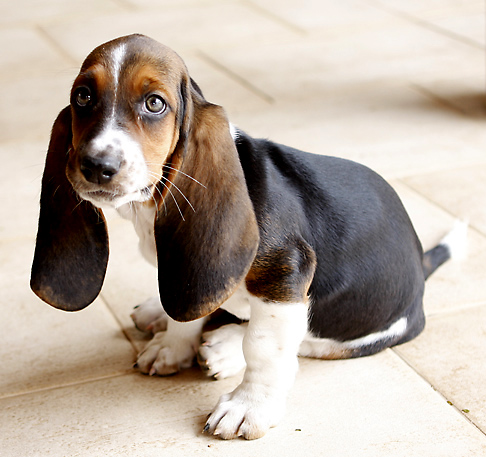
\includegraphics[width=20mm]{./figures/basset-hound.jpeg}
      \caption{\centering This is a [DOG]. \\ \tiny{Image from Wikipedia, \href{https://commons.wikimedia.org/w/index.php?curid=32270218}{Link}}}
    \end{figure}
    \column{.5\textwidth} 
    \begin{figure}
      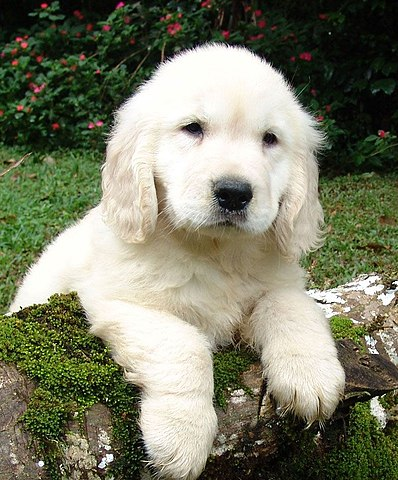
\includegraphics[width=20mm]{./figures/golden-retriever-puppy.jpeg}
      \caption{\centering Is this a [DOG]? \\ \tiny{Image from Wikipedia, \href{https://commons.wikimedia.org/w/index.php?curid=18521767}{Link}}}
    \end{figure}
    \vspace{-0.5cm}
    % \centering 
    \small{\emph{Prompt}: Is this a [DOG]?\\
    \emph{Expected Answer}: Yes}
  \end{columns}
\end{frame}
\note{
- Few-shot transfer is different from traditional machine learning that requires many examples \\
- The model doesn't actually learn in the traditional sense; it leverages knowledge from pre-training \\
- In this example, we show the model one example of a dog (a basset hound) and ask it to identify another dog \\
- This works because the model already knows what dogs look like from pre-training \\
- The quotation marks around 'learns' emphasize that it's not learning from scratch. I like to think of it as somehow narrowing the tree of possible responses from a point \\
}


\subsection{Motivation}
\begin{frame}{Motivation}
\framesubtitle{Few-Shot Transfer}
  \vspace{-1em}
  \begin{columns}[T]
    \column{0.5\textwidth}
      \centering \emph{Fine-tuning}
      \begin{itemize}
        \item Requires significant computational resources, modifies model parameters
        \item Needs \emph{large(r) amounts} of \emph{labeled data}
        \item Can lead to catastrophic forgetting
        \item Refers to fine-tuning a pre-trained / instruction-tuned model on a specific task
      \end{itemize}
    \column{0.5\textwidth}
    \centering \emph{Few-shot Transfer}
    \begin{itemize}
        \item Uses \emph{`few' examples} or natural language \emph{descriptions}
        \item No model parameters are updated
        \item Potentially more practical for real-world applications~\footfullciteieee{Brown2020}
        \item Can be less effective for complex tasks
    \end{itemize}
  \end{columns}
\end{frame}
\note{
- Fine-tuning is the traditional approach for adapting pre-trained models to new tasks \\
- For VLMs, fine-tuning can require multiple high-end GPUs and days of compute time \\
- Catastrophic forgetting means the model may lose previously learned capabilities \\
- Few-shot transfer is much more efficient - we can use the model "as is" \\
- An important distinction: fine-tuning modifies the model weights, few-shot transfer doesn't \\
- The trade-off is that few-shot performance may not match fine-tuned performance for complex tasks \\
}


\subsection{Problem Statement}
\begin{frame}{Problem Statement}
\framesubtitle{Dataset Labeling for Computer Vision Tasks}
  \textbf{Challenge:} Creating labeled datasets to train specialized models for computer vision tasks is \emph{time-consuming} and \emph{expensive}~\footfullciteieee{Deng2009}, but VLMs are generalizable
  \vspace{0.5em}

  \textbf{Constraint:} However, VLMs are too \emph{computationally intensive} for direct deployment on resource-constrained environments (e.g., robots)
  \vspace{0.5em}
    
  \textbf{Opportunity:} VLMs could potentially automate label generation (\emph{pseudolabels}) to train \emph{downstream} models
  \vspace{1.2em}

  \centering \textbf{Research Question:} Can VLMs be transferred to generate \emph{pseudolabels} for computer vision tasks to train \emph{lightweight} downstream models?
  \blfootnote{\vspace{0.05em}}
\end{frame}
\note{
- The annotation of the ImageNet dataset required crowdsourcing to be feasible \\
- Specialized datasets like medical imaging can be even more expensive and require expert annotators \\
- VLMs require significant computational resources - multiple high-end GPUs with significant amounts of memory \\
- Most robots have limited computational capabilities - often a single low-power GPU or CPU \\
- Pseudolabels are automatically generated annotations that can be used in place of human-created labels \\
- The key insight: we don't need to deploy the large model - we use it to train a smaller, more efficient model \\
}


% \subsection{Proposed Approach}
\begin{frame}{Proposed Approach}
\framesubtitle{Evaluating VLMs for Pseudolabel Generation}
  \textbf{Approach:} Evaluate VLMs on generating \emph{accurate pseudolabels} under various \emph{zero-shot} and \emph{few-shot} transfer conditions
  \vspace{0.3em}
    
  \begin{columns}[T]
    \column{0.55\textwidth}
      \centering \textbf{Key Research Aspects}
      \begin{enumerate}
        \item How does the \emph{number of examples} (few-shot vs. zero-shot) affect pseudolabel quality?
        \item What are the \emph{computational requirements} for practical application?
        \item How effective are the \emph{downstream models} trained on pseudolabels?
      \end{enumerate}

    \column{0.45\textwidth}
    \begin{figure}
      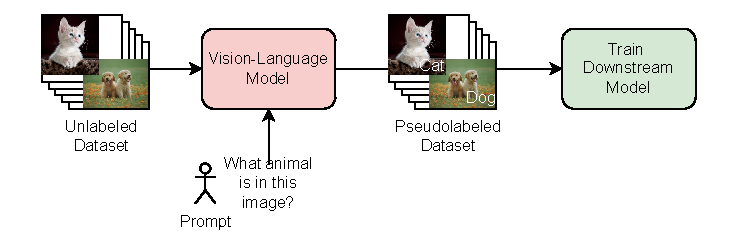
\includegraphics[width=\textwidth]{figures/vlm_transfer_downstream.pdf}
      \caption{\centering Using VLMs to generate pseudolabels for downstream model training}
    \end{figure}
  \end{columns}
\end{frame}
\note{
- Zero-shot means only describing the task in natural language; few-shot means providing examples \\
- We tested multiple prompting strategies to find the most effective approach \\
- We examined both common visual tasks (CIFAR-10) and specialized tasks (dermatology) to see if few-shot transfer is generalizable \\
- This design helps us understand when VLMs can be reliably transferred for automatic labeling \\
- For computational requirements, we measured inference time, memory usage, and scaling properties \\
- Downstream models were evaluated against models trained on ground truth labels \\
}


\section{Related Work}
\subsection{Background}
\begin{frame}{Related Work}
\framesubtitle{Development and Classes of Vision-Language Models}
  \vspace{-1em}
  \begin{columns}[T]
    \column{\customcolumnwidth}
    \textbf{VLM Classes}
    \vspace{-0.4em}
    \begin{itemize}
      \item \emph{Alignment models}: Generate unified text-image embeddings (CLIP~\footfullciteieee{Radford2021}, FLAVA) \vspace{-0.2em}
      \item \emph{Generative models}: Generate text conditioned on multimodal inputs (Flamingo, Frozen~\footfullciteieee{Tsimpoukelli2021}, MiniCPM~\footfullciteieee{Yao2024}, GPT-4o, Claude, etc.)
    \end{itemize}
    \column{\customcolumnwidth}
    \textbf{Architectural Approaches}
    \vspace{-0.4em}
    \begin{itemize}
      \item \emph{Towered}: Separate vision and language models with adapters
      \item \emph{Unified}: Single model processing both modalities "early on"~\footfullciteieee{ChameleonTeam2024}
    \end{itemize}
    \textbf{Key Insight}: Enables framing vision tasks as text generation~\footfullciteieee{Cho2021}, enabling streamlined task transfer
  \end{columns}
\end{frame}
\note{
- Vision-Language Models (VLMs) have progressed significantly since the introduction of CLIP \\
- Alignment models, such as CLIP, are designed to learn joint representations but do not generate textual outputs \\
- In contrast, generative models are capable of producing text responses based on visual inputs \\
- The Frozen model pioneered the approach of freezing the language model (LLM) while solely training the vision encoder \\
- Contemporary VLMs often incorporate separate pre-trained components for vision and language, connected through adapters or connectors \\
- Additionally, unified architectures that process both modalities simultaneously have emerged, enhancing the integration of vision and language tasks \\
- A pivotal advancement facilitating few-shot transfer is the conceptualization of vision tasks as text generation tasks \\
- This paradigm allows us to articulate tasks using natural language, eliminating the need for specialized architectures \\
- The rapid evolution of this field has led to the emergence of models like GPT-4o, which can comprehend and reason about complex visual scenarios \\
}


\begin{frame}{Related Work}
\framesubtitle{Transfer Learning \& Adaptation Techniques}
  \vspace{-1em}
  \begin{columns}[T]
    \column{\customcolumnwidth}
      \textbf{Prompting Techniques}: Crafting prompts to improve task performance~\footfullciteieee{Liu2023}
      \begin{itemize}
        \item In-context learning: Providing examples in context~\footfullciteieee{Brown2020}
        \item Chain-of-thought prompting for complex reasoning~\footfullciteieee{Wei2022}
      \end{itemize}
    \column{\customcolumnwidth}
      \textbf{Parameter-Efficient Fine-Tuning}: Typically requires more examples than few-shot regime
      \begin{itemize}
        \item Prefix-tuning: Optimizing task-specific prompt vectors~\footfullciteieee{Li2021}
        \item Low-Rank Adaptation (LoRA)~\footfullciteieee{Hu2021}: decomposes weight updates into smaller trainable matrices
      \end{itemize}
  \end{columns}
\end{frame}
\note{
- Prompting techniques are crucial for adapting models to new tasks without retraining \\
- In-context learning allows models to learn from examples without parameter updates \\
- Chain-of-thought prompting helps models break down complex tasks into simpler steps \\
- Parameter-efficient fine-tuning methods like prefix-tuning are valuable for low-resource settings \\
- These techniques are less explored in VLMs compared to NLP models \\
- Our research contributes by evaluating these methods in the context of VLMs for dataset annotation \\
}


\begin{frame}{Related Work}
\framesubtitle{Applications and Datasets}
  \vspace{-1em}
  \begin{columns}[T]
    \column{\customcolumnwidth}
      \textbf{Applicability of VLMs}
      \vspace{-0.4em}
      \begin{itemize}
        \item Large-scale pre-training enables generalization to various tasks
        \item Traditional DNNs trained for specific tasks
      \end{itemize}
      \textbf{LLMs for Data Annotation}
      \vspace{-0.4em}
      \begin{itemize}
        \item LLMs used to generate multimodal instruction-following data~\footfullciteieee{Liu2023a}
        \item Seen to outperform crowd-workers in data annotation tasks~\footfullciteieee{Gilardi2023}
      \end{itemize}
    \column{\customcolumnwidth}
      \textbf{Key Datasets}:
      Various datasets exist for various vision tasks.
      \begin{itemize}
        \item ImageNet, CIFAR-10~\footfullciteieee{Krizhevsky2009}: Object recognition
        \item Microsoft COCO: Detection, segmentation, captioning
        \item Derm7Pt~\footfullciteieee{Kawahara2019}: Specialized dermatology dataset
        \item MVTec: Anomaly detection
      \end{itemize}
  \end{columns}
\end{frame}
\note{
- VLMs are used in a wide range of vision tasks, leveraging their ability to generalize from large-scale pre-training \\
- Traditional DNNs are typically trained on specific datasets for specific tasks, limiting their generalization \\
- LLMs have been used to generate multimodal instruction-following data to train VLMs, enhancing dataset creation \\
- LLMs have been seen to outperform human annotators, providing more consistent and scalable data annotation \\
- Key datasets like ImageNet and CIFAR-10 are benchmarks for evaluating model performance on object recognition \\
- Specialized datasets like Derm7Pt are crucial for testing models on domain-specific tasks \\
- Our research leverages these datasets to evaluate the effectiveness of VLMs in generating pseudolabels for downstream tasks \\
}


\subsection{Research Gaps and Limitations}
\begin{frame}{Research Gaps and Limitations}
\framesubtitle{What do we address, and what could hinder our work?}
  \vspace{-1em}
  \begin{columns}[T]
    \column{\customcolumnwidth}
      \textbf{Gaps Addressed in Our Work}
      \begin{itemize}
        \item Few-shot transfer of VLMs less explored than NLP counterparts~\footfullciteieee{Liu2023}
        \item Dataset annotation applications~\footfullciteieee{Tan2024}:
        \begin{itemize}
          \item Use of VLMs for dataset annotation less explored
          \item Analysis of downstream vision models from VLM-generated pseudolabels
        \end{itemize}
      \end{itemize}
    \column{\customcolumnwidth}
      \textbf{Known VLM Limitations}
      \begin{itemize}
        \item Systematic shortcomings in visual reasoning, spatial relationships, and perspective~\footfullciteieee{Tong2024}
        \item Inherited LLM issues~\footfullciteieee{Li2023c} such as hallucinations, ungrounded reasoning, prior biases~\footfullciteieee{Chochlakis2024}
      \end{itemize}
  \end{columns}
\end{frame}
\note{
- Few-shot transfer capabilities of VLMs are less studied compared to LLMs in NLP \\
- Most VLM research focuses on zero-shot or fine-tuning approaches \\
- Our work systematically evaluates VLMs for dataset annotation: \\
  - Comprehensive evaluation of different prompting strategies \\
  - Analysis of pseudolabel quality and consistency \\
  - Impact on downstream model performance \\
- We acknowledge important VLM limitations: \\
  - Difficulty with spatial relationships and perspective \\
  - Inherited issues from LLMs like hallucinations \\
  - Biases from pre-training data making model ignore visual context \\
- These limitations highlight areas needing further research \\
}


\section{Methodology}
\subsection{Experimental Setup}
\begin{frame}{Experimental Setup}
  % Content will be added later
\end{frame}

\subsection{Datasets}
\begin{frame}{Datasets}
  % Content will be added later
\end{frame}

\subsection{Models and Prompting Strategies}
\begin{frame}{Models and Prompting Strategies}
  % Content will be added later
\end{frame}

\section{Evaluation}
\subsection{CIFAR-10 Experiments}
\begin{frame}{CIFAR-10 Experiments}
\framesubtitle{A General Image Classification Task}
  \vspace{-1em}
  \begin{columns}[T]
    \column{\customcolumnwidth}
      \textbf{Experimental Setup}
      \begin{itemize}
        \item Four VLMs evaluated:
        \begin{itemize}
          \item Pixtral 12B
          \item InternVL2
          \item MiniCPM v2.6
          \item Phi-3.5 Vision Instruct
        \end{itemize}
        \item Prompting strategies:
        \begin{itemize}
          \item Zero-shot (0-shot, 0.5-shot, chain-of-thought)
          \item Few-shot (1-16 examples, with and without textual prompts)
        \end{itemize}
      \end{itemize}
    \column{\customcolumnwidth}
      \textbf{Key Findings}
      \begin{itemize}
        \item Zero-shot performance:
        \begin{itemize}
          \item Consistent across prompting strategies
          \item Reasoning requirements decreased accuracy by 10-15\%
        \end{itemize}
        \item Few-shot insights:
        \begin{itemize}
          \item Performance peaks at 4-8 examples
          \item Super-linear increase in resource usage
          \item Prompting improves low-shot scenarios
        \end{itemize}
      \end{itemize}
  \end{columns}
\end{frame}
\note{
- Evaluated four state-of-the-art VLMs on CIFAR-10 image classification \\
- Zero-shot experiments showed consistent performance across different prompting strategies \\
- Adding reasoning requirements actually decreased performance by 10-15\% due to format constraints and the limitations of some VLMs in following instructions \\
- Few-shot performance varied by model: Pixtral and InternVL2 showed improvements up to 8 examples \\
- MiniCPM and Phi-3.5 peaked earlier at 4-6 examples \\
- Resource usage increased super-linearly with number of examples \\
- Memory usage patterns varied: Pixtral showed super-linear increase, MiniCPM remained constant \\
- Processing time increased dramatically: 2 examples ~10x, 4 examples ~20x, 8 examples 30-50x longer than zero-shot \\
- Downstream models trained on pseudolabels often outperformed the VLMs themselves \\
}

\subsection{Downstream Model Analysis}
\begin{frame}{Downstream Model Analysis}
\framesubtitle{Performance Characteristics and Insights}
  \vspace{-1em}
  \begin{columns}[T]
    \column{\customcolumnwidth}
      \textbf{Performance Characteristics}
      \begin{itemize}
        \item Downstream models outperformed VLMs, possibly due to:
        \begin{itemize}
          \item Pre-trained ResNet-18 model~\footfullciteieee{He2016}
          \item Focus on pattern recognition compared to image-text modeling
        \end{itemize}
        % Rework this section, it is not clear at all
        \item Label quality vs. dataset size:
        \begin{itemize}
          \item Quality more crucial than quantity
          \item 90\% VLM accuracy threshold
        \end{itemize}
      \end{itemize}
    \column{\customcolumnwidth}
      \textbf{Key Insights}
      \begin{itemize}
        \item Weak dependence of performance on shot count
        \item Embracing noise: label smoothing improved performance by \(\sim\)1\%
        \item Practical implications:
        \begin{itemize}
          \item Zero/low-shot approaches sufficient
          \item Simple prompts more effective
          \item High resilience to label noise
        \end{itemize}
      \end{itemize}
  \end{columns}
\end{frame}
\note{
- Downstream models consistently outperformed VLMs due to ImageNet pre-training and focus on pattern recognition \\
- Performance showed weak dependence on number of examples used in VLM predictions \\
- Models maintained good performance even with lower-quality labels from 1-shot experiments \\
- Label quality proved more important than dataset size in training \\
- Models trained on limited but accurate ground truth labels performed better until VLM accuracy reached ~90\% \\
- Practical finding: zero-shot or low-shot (1-2 examples) with prompting is most efficient implementation strategy \\
- Higher shot counts showed diminishing returns despite increased computational costs \\
- Downstream models showed remarkable resilience to label quality, suggesting practical utility even with imperfect data \\
}


\subsection{Specialized Domain (Derm7Pt) Experiments}
\begin{frame}{Dermatology Experiments}
  \vspace{-1em}
  \begin{columns}[T]
    \column{\customcolumnwidth}
      \textbf{Experimental Setup}
      \begin{itemize}
        \item Five VLMs evaluated:
        \begin{itemize}
          \item Pixtral 12B, InternVL2
          \item MiniCPM v2.6, Phi-3.5
          \item Biomedical Multimodal Model (domain-specific, fine-tuned model)
        \end{itemize}
        \item Two experiment types:
        \begin{itemize}
          \item Direct diagnosis of condition
          \item Structured feature understanding (7-point checklist with category-specific prompts)
        \end{itemize}
      \end{itemize}
    \column{\customcolumnwidth}
      \textbf{Evaluation Framework}
      \begin{itemize}
        \item Multiple image modalities:
        \begin{itemize}
          \item Dermoscopic images (standardized)
          \item Clinical images (inconsistent, optional)
        \end{itemize}
        \item Prompting strategies:
        \begin{itemize}
          \item Zero-shot with/without reasoning
          \item Few-shot (1-8 examples with and without textual prompts)
        \end{itemize}
      \end{itemize}
    \end{columns}
\end{frame}

\begin{frame}{Dermatology Experiments}
\framesubtitle{Key Findings}
  \begin{columns}[T]
    \column{\customcolumnwidth}
      \textbf{Performance Patterns}
      \begin{itemize}
        \item Most models near random-guess accuracy
        \item Domain-specific model struggled significantly, with poor instruction following
        \item Clinical images often degraded performance
        \item Resource usage with clinical images:
        \begin{itemize}
          \item Memory: 1-1.75x increase
          \item Time: 1.5-2.5x longer processing
        \end{itemize}
      \end{itemize}
    \column{\customcolumnwidth}
      \textbf{Key Challenges}
      \begin{itemize}
        \item Limited pre-training knowledge
        \item Multi-modal integration issues
        \item Performance degradation with:
        \begin{itemize}
          \item Increased examples
          \item Added reasoning requirements
          \item Multiple image modalities (addition of clinical images)
        \end{itemize}
      \end{itemize}
  \end{columns}
\end{frame}

\begin{frame}{Dermatology Experiments}
\framesubtitle{Structured vs Direct Diagnosis}
  \begin{columns}[T]
    \column{0.5\textwidth}
      \textbf{Direct Diagnosis Approach}
      \begin{itemize}
        \item Zero-shot baseline:
          \begin{itemize}
            \item Only Pixtral 12B above random
            \item Reasoning decreased performance
          \end{itemize}
        \item Few-shot performance:
          \begin{itemize}
            \item Some improvement over zero-shot
            \item Diminishing returns with examples
          \end{itemize}
      \end{itemize}
    \column{0.5\textwidth}
      \textbf{Structured Prompting}
      \begin{itemize}
        \item Seven-point checklist categories
        \item Performance patterns:
          \begin{itemize}
            \item Generally inferior to zero-shot
            \item Peak at 2-4 examples for most models
            \item Limited benefit from task-specific info
          \end{itemize}
      \end{itemize}
  \end{columns}
\end{frame}
\note{
- The Derm7Pt experiments revealed significant challenges in applying VLMs to specialized medical tasks \\
- Most models performed at or around random-guessing accuracy, indicating fundamental limitations \\
- Adding clinical images alongside dermoscopic images often degraded performance \\
- Even the domain-specific Biomedical Multimodal Model struggled significantly \\
- Resource requirements increased substantially with experiment complexity \\
- Direct diagnosis showed some promise with few-shot learning, while structured prompting was generally less effective \\
- These findings suggest current VLMs need significant improvements for specialized medical tasks \\
- The results highlight the importance of pre-existing task knowledge in few-shot learning success \\
}

\begin{frame}{Dermatology Experiments}
\framesubtitle{Implications and Conclusions}
  \begin{columns}[T]
    \column{0.5\textwidth}
      \textbf{Key Insights}
      \begin{itemize}
        \item Pre-training knowledge crucial:
          \begin{itemize}
            \item Poor performance on specialized tasks
            \item Transferability to specialized domains not guaranteed
          \end{itemize}
        \item Architectural considerations:
          \begin{itemize}
            \item Model size \(\neq\) performance
            \item Multi-modal integration challenges
          \end{itemize}
      \end{itemize}
    \column{0.5\textwidth}
      \textbf{Future Directions}
      \begin{itemize}
        \item Specialized training needed:
          \begin{itemize}
            \item Domain-specific pre-training
            \item Better multi-modal integration
          \end{itemize}
        \item Practical considerations:
          \begin{itemize}
            \item Simpler prompting strategies
            \item Resource-performance trade-offs
            \item Task-specific evaluation metrics
          \end{itemize}
      \end{itemize}
  \end{columns}
\end{frame}
\note{
- Context length and memory limitations restricted few-shot experiments to limited examples and constrained larger models \\
- Observed trends already show limited/degraded performance scaling with higher number of examples \\
- Poor performance on specialized domains suggests models rely more on pre-trained priors than learning new capabilities \\
- Promising research directions include investigating domain-specific pre-training strategies \\
- More efficient VLM architectures needed for scalable high-resolution multi-image processing \\
- Beyond classification, future work could explore VLM application for image captioning and segmentation \\
- Improved prompting strategies needed to enhance visual grounding and reasoning capabilities \\
}

\subsection{Compute Analysis}
\begin{frame}{Compute Analysis}
\framesubtitle{Analysis of Memory and Processing Time}
  \vspace{-1em}
  \begin{columns}[T]
    \column{\customcolumnwidth}
      \textbf{Memory Usage Patterns}
      \begin{itemize}
        \item Model-dependent scaling:
        \begin{itemize}
          \item Pixtral 12B: Super-linear increase
          \item InternVL2, Phi-3.5: Linear scaling
          \item MiniCPM: Near-constant (perceiver-resampler)
        \end{itemize}
        \item Clinical images (dermatology experiments): 1-1.75x increase
        \item Less than the expected quadratic scaling for pure transformers~\footfullciteieee{Vaswani2017}
      \end{itemize}
    \column{\customcolumnwidth}
      \textbf{Processing Time Impact}
      \begin{itemize}
        \item Super-linear increase with examples (compared to zero-shot):
        \vspace{-1em}
        \begin{itemize}
          \item 2 examples: \(\sim\)10x longer
          \item 4 examples: \(\sim\)20x longer
          \item 8 examples: 30-50x longer
        \end{itemize}
        \item Reasoning requirements: 10-35\% longer
        \item Clinical images (dermatology experiments): 1.5-2.5x longer
      \end{itemize}
  \end{columns}
\end{frame}
\note{
- Memory usage patterns vary significantly between model architectures \\
- Pixtral 12B shows super-linear memory scaling with number of examples, likely due to pure transformer architecture \\
- InternVL2 and Phi-3.5 show more manageable linear scaling patterns \\
- MiniCPM's perceiver-resampler architecture enables near-constant memory usage regardless of examples \\
- Clinical images (additional images) increase memory usage by 1-1.75x \\
- Processing time increases dramatically with number of examples used \\
- Adding reasoning requirements (e.g., chain-of-thought) increases processing time by 10-35\% due to the generation of more output tokens \\
- Clinical images take 1.5-2.5x longer to process due to increased number of images and complexity \\
- These patterns align with theoretical expectations for optimized transformer architectures, and are lower than the expected quadratic scaling \\
}


\begin{frame}{Compute Analysis}
\framesubtitle{Practical Implications}
  \vspace{-1em}
  \begin{columns}[T]
    \column{\customcolumnwidth}
      \textbf{Resource-Performance Trade-offs}
      \begin{itemize}
        \item Diminishing returns with examples:
        \vspace{-1em}
        \begin{itemize}
          \item Performance peaks at 4-8 examples
          \item Resource costs grow super-linearly
        \end{itemize}
        \item Architecture and model pre-training considerations:
        \begin{itemize}
          \item Perceiver-resampler based models more efficient
          \item Models pre-trained on multi-image, multi-turn conversation may perform better
          \item Larger model size \(\nRightarrow\) better performance
        \end{itemize}
      \end{itemize}
    \column{\customcolumnwidth}
      \textbf{Recommendations}
      \begin{itemize}
        \item Optimal approach:
        \begin{itemize}
          \item Zero-shot or 1-2 shot prompting
          \item Avoid reasoning requirements
          \item Single-image-per-turn processing when possible
        \end{itemize}
      \end{itemize}
  \end{columns}
\end{frame}
\note{
- Resource costs grow much faster than performance improvements with additional examples \\
- Perceiver-resampler architectures (like in MiniCPM) show better memory efficiency \\
- However, there may be a trade-off between resource efficiency and model performance \\
- Zero-shot or low-shot (1-2 examples) provides best balance of performance vs. resources \\
- Avoiding reasoning requirements saves significant processing time without major performance loss \\
- Multi-image processing (e.g., clinical + dermoscopic) significantly impacts resources \\
- Architecture choice crucial for scaling to larger datasets or more complex tasks \\
- These findings help inform practical deployment strategies for VLMs in real applications \\
}


\section{Conclusions}
% \subsection{Key Findings}
\begin{frame}{Key Findings}
  % Content will be added later
\end{frame}

% \subsection{Limitations and Future Work}
\begin{frame}{Limitations and Future Work}
    \begin{columns}[T]
        \column{\customcolumnwidth}
            \textbf{Technical Limitations}
            \begin{itemize}
                \item Context length and memory constraints
                \begin{itemize}
                    \item Limited number of examples
                    \item High-resolution image limitations
                    \item Restricted use of larger models
                \end{itemize}
                \item Limited / degraded performance scaling with number of examples
                \item Limited generalization to specialized domains
                \item Our findings may not generalize to all vision tasks
            \end{itemize}
        \column{\customcolumnwidth}
            \textbf{Future Research Directions}
            \begin{itemize}
                \item Generalizable domain-specific pre-training strategies
                \item More efficient VLM architectures for multi-image processing
                \item Improving prompting strategies and visual grounding~\footfullciteieee{Yang2023}
                \item Extending investigation to other vision tasks:
                \begin{itemize}
                    \item Image captioning
                    \item Segmentation
                \end{itemize}
            \end{itemize}
    \end{columns}
\end{frame}
\note{
- Context length and memory limitations restricted few-shot experiments to limited examples and constrained larger models \\
- Observed trends already show limited/degraded performance scaling with higher number of examples \\
- Poor performance on specialized domains suggests models rely more on pre-trained priors than learning new capabilities \\
- Promising research directions include investigating domain-specific pre-training strategies \\
- More efficient VLM architectures needed for scalable high-resolution multi-image processing \\
- Beyond classification, future work could explore VLM application for image captioning and segmentation \\
- Improved prompting strategies needed to enhance visual grounding and reasoning capabilities \\
}

% \section{Q\&A}
\begin{frame}{Thank You!}
  \centering
  \vfill
  {\LARGE Questions?}
  \vfill
  \raggedright\textbf{Contact:}
  \begin{itemize}
    \item shinas.shaji@smail.inf.h-brs.de
    \item shinas.shaji@iais.fraunhofer.de
  \end{itemize}
  \vfill
\end{frame}

\end{document}
